% APÊNDICES------------------------------------------------

\begin{apendicesenv}
\partapendices

% Primeiro apêndice---------------------------------------
\chapter{Repositório no GitHub} % Edite para alterar o título deste apêndice
\label{apendice_1}

\noindent Link repositório:\\
\href{https://github.com/Oseiasdfarias/Projeto\_Tcc\_Oseias\_Oficial}{https://github.com/Oseiasdfarias/Projeto\_Tcc\_Oseias\_Oficial}\\

\noindent Link Site de Documentação:\\ \href{https://oseiasdfarias.github.io/Projeto\_Tcc\_Oseias\_Oficial/}{https://oseiasdfarias.github.io/Projeto\_Tcc\_Oseias\_Oficial}\\

\begin{figure}[!h]
	\centering
	\caption{Repositório no GitHub.}
	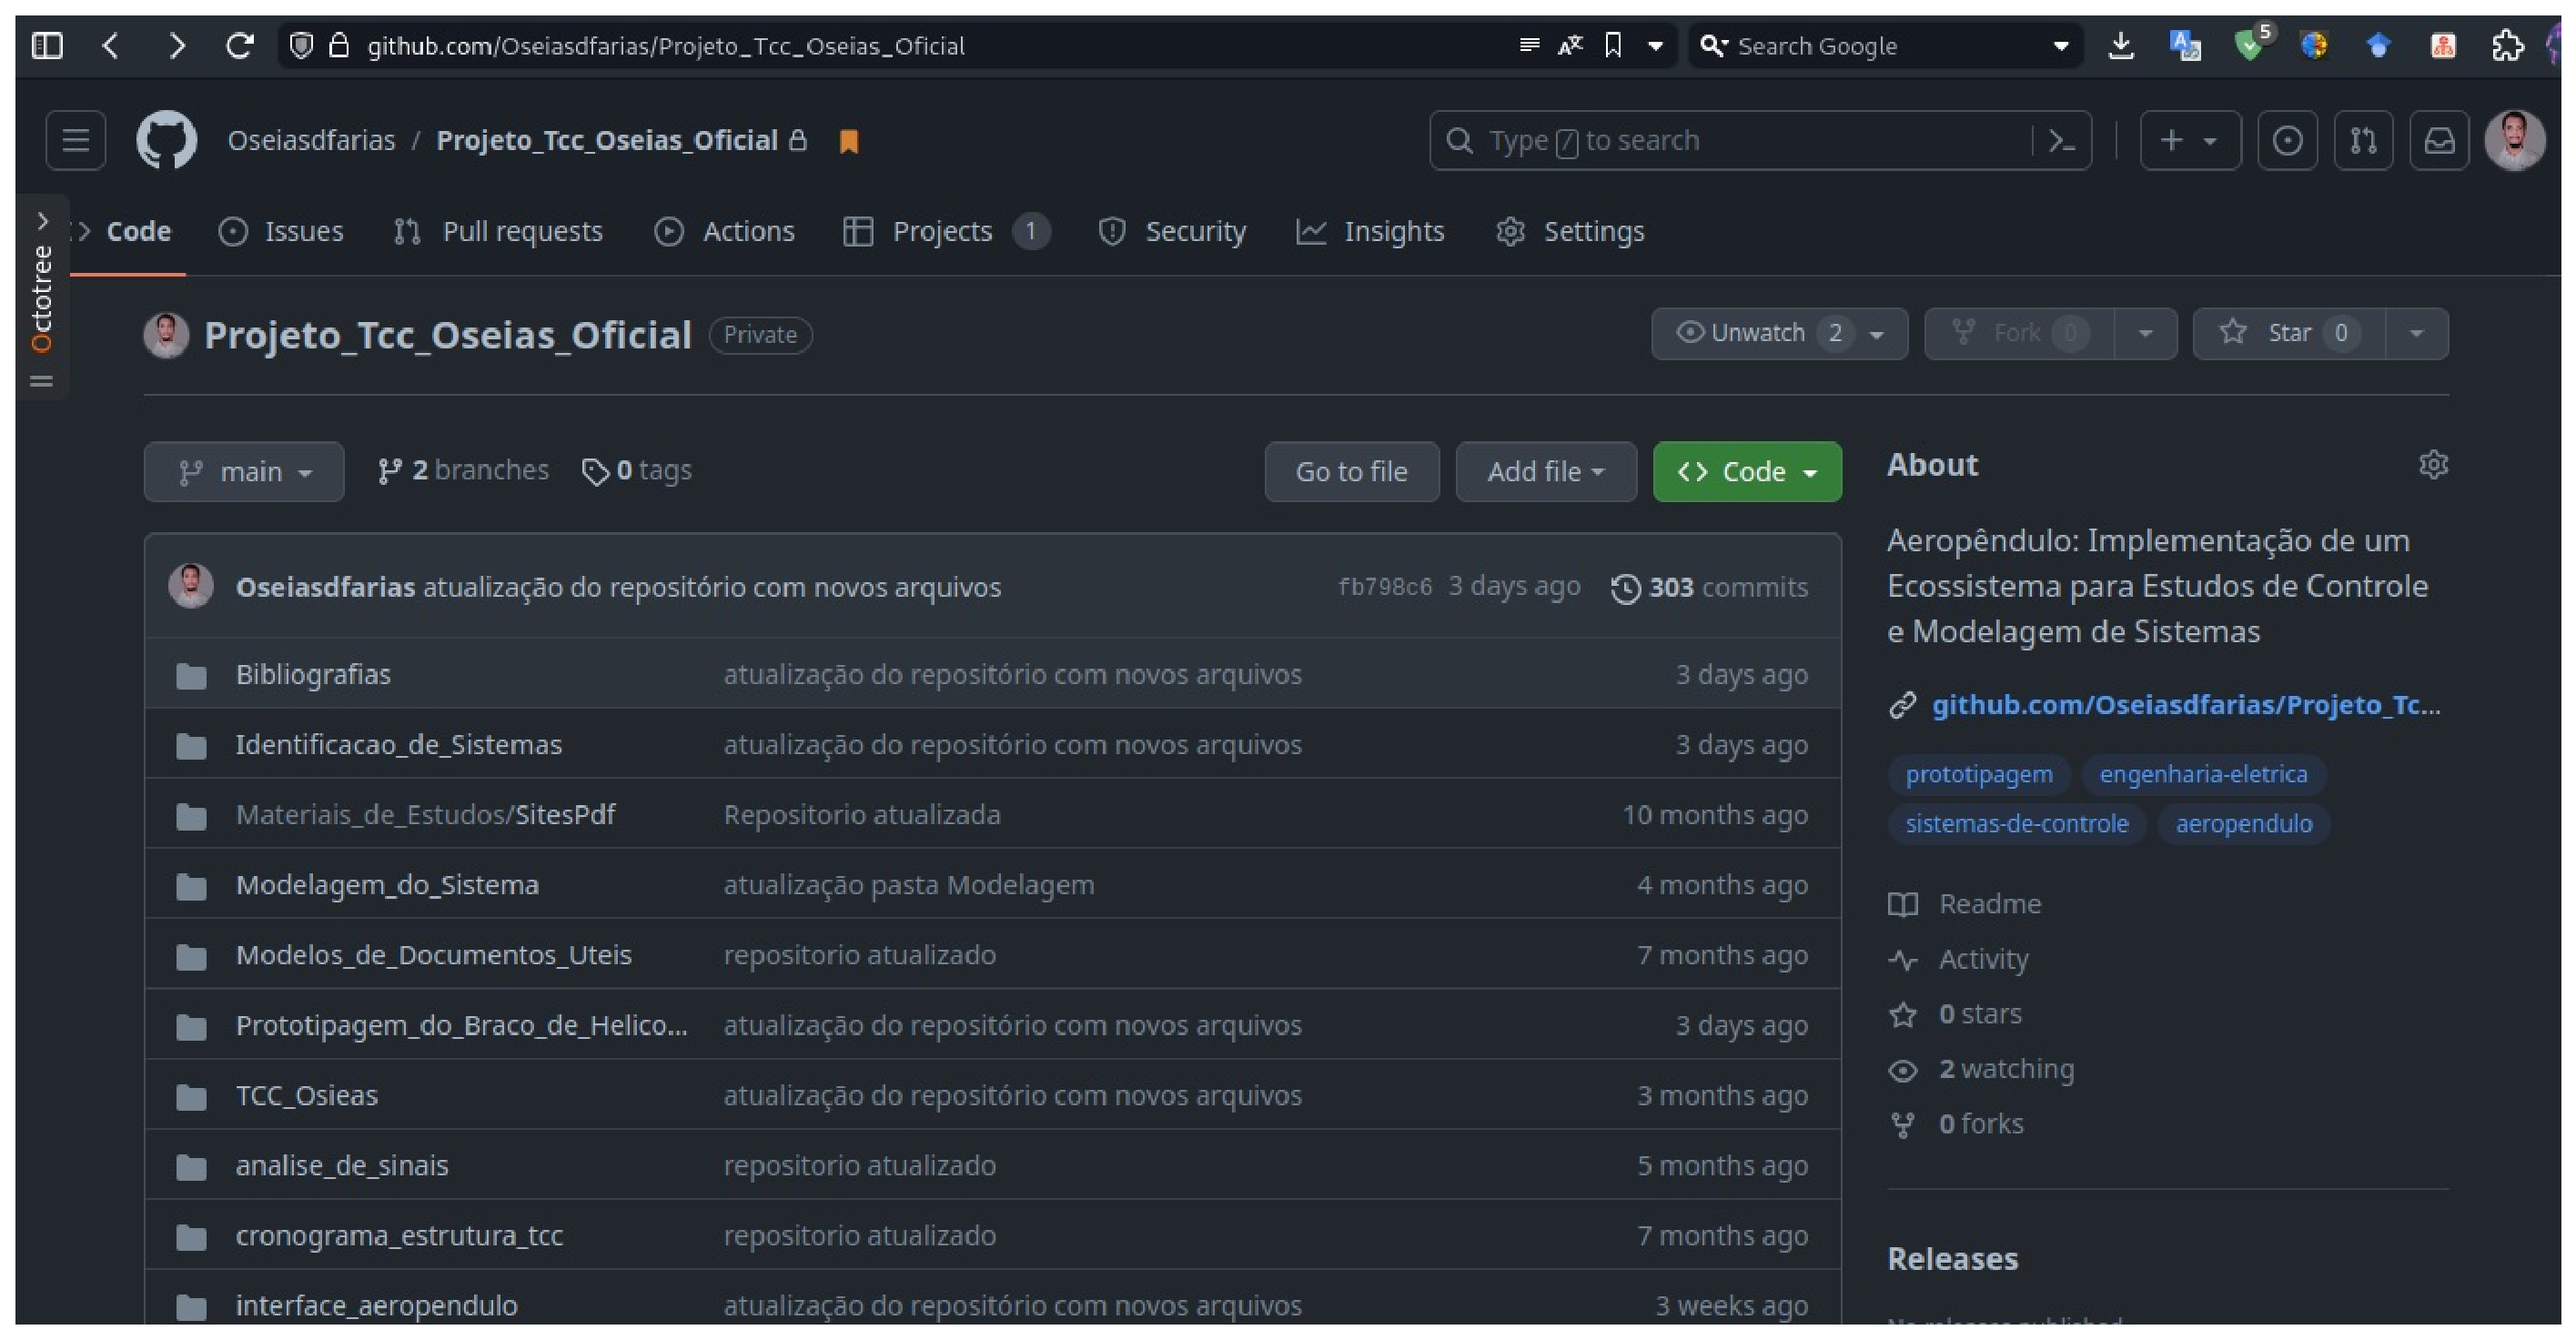
\includegraphics[width=1.0\textwidth]{utils/repo_github.eps}
	\caption*{Fonte: elaborado pelo autor (2023).}
	\label{fig3:image_27}
\end{figure}


% Novo apêndice----------------------------------------------------------------
%\chapter{Nome do outro apêndice}
%\label{chap:apendiceB}
%
%conteúdo do novo apêndice

\end{apendicesenv}
